% Options for packages loaded elsewhere
\PassOptionsToPackage{unicode}{hyperref}
\PassOptionsToPackage{hyphens}{url}
%
\documentclass[
]{article}
\usepackage{lmodern}
\usepackage{amssymb,amsmath}
\usepackage{ifxetex,ifluatex}
\ifnum 0\ifxetex 1\fi\ifluatex 1\fi=0 % if pdftex
  \usepackage[T1]{fontenc}
  \usepackage[utf8]{inputenc}
  \usepackage{textcomp} % provide euro and other symbols
\else % if luatex or xetex
  \usepackage{unicode-math}
  \defaultfontfeatures{Scale=MatchLowercase}
  \defaultfontfeatures[\rmfamily]{Ligatures=TeX,Scale=1}
\fi
% Use upquote if available, for straight quotes in verbatim environments
\IfFileExists{upquote.sty}{\usepackage{upquote}}{}
\IfFileExists{microtype.sty}{% use microtype if available
  \usepackage[]{microtype}
  \UseMicrotypeSet[protrusion]{basicmath} % disable protrusion for tt fonts
}{}
\makeatletter
\@ifundefined{KOMAClassName}{% if non-KOMA class
  \IfFileExists{parskip.sty}{%
    \usepackage{parskip}
  }{% else
    \setlength{\parindent}{0pt}
    \setlength{\parskip}{6pt plus 2pt minus 1pt}}
}{% if KOMA class
  \KOMAoptions{parskip=half}}
\makeatother
\usepackage{xcolor}
\IfFileExists{xurl.sty}{\usepackage{xurl}}{} % add URL line breaks if available
\IfFileExists{bookmark.sty}{\usepackage{bookmark}}{\usepackage{hyperref}}
\hypersetup{
  pdftitle={TBASS: A Robust Adaptation of Bayesian Adaptive Spline Surfaces},
  pdfauthor={Andy A. Shen, Kellin N. Rumsey, Devin C. Francom},
  hidelinks,
  pdfcreator={LaTeX via pandoc}}
\urlstyle{same} % disable monospaced font for URLs
\usepackage[margin=1in]{geometry}
\usepackage{color}
\usepackage{fancyvrb}
\newcommand{\VerbBar}{|}
\newcommand{\VERB}{\Verb[commandchars=\\\{\}]}
\DefineVerbatimEnvironment{Highlighting}{Verbatim}{commandchars=\\\{\}}
% Add ',fontsize=\small' for more characters per line
\usepackage{framed}
\definecolor{shadecolor}{RGB}{248,248,248}
\newenvironment{Shaded}{\begin{snugshade}}{\end{snugshade}}
\newcommand{\AlertTok}[1]{\textcolor[rgb]{0.94,0.16,0.16}{#1}}
\newcommand{\AnnotationTok}[1]{\textcolor[rgb]{0.56,0.35,0.01}{\textbf{\textit{#1}}}}
\newcommand{\AttributeTok}[1]{\textcolor[rgb]{0.77,0.63,0.00}{#1}}
\newcommand{\BaseNTok}[1]{\textcolor[rgb]{0.00,0.00,0.81}{#1}}
\newcommand{\BuiltInTok}[1]{#1}
\newcommand{\CharTok}[1]{\textcolor[rgb]{0.31,0.60,0.02}{#1}}
\newcommand{\CommentTok}[1]{\textcolor[rgb]{0.56,0.35,0.01}{\textit{#1}}}
\newcommand{\CommentVarTok}[1]{\textcolor[rgb]{0.56,0.35,0.01}{\textbf{\textit{#1}}}}
\newcommand{\ConstantTok}[1]{\textcolor[rgb]{0.00,0.00,0.00}{#1}}
\newcommand{\ControlFlowTok}[1]{\textcolor[rgb]{0.13,0.29,0.53}{\textbf{#1}}}
\newcommand{\DataTypeTok}[1]{\textcolor[rgb]{0.13,0.29,0.53}{#1}}
\newcommand{\DecValTok}[1]{\textcolor[rgb]{0.00,0.00,0.81}{#1}}
\newcommand{\DocumentationTok}[1]{\textcolor[rgb]{0.56,0.35,0.01}{\textbf{\textit{#1}}}}
\newcommand{\ErrorTok}[1]{\textcolor[rgb]{0.64,0.00,0.00}{\textbf{#1}}}
\newcommand{\ExtensionTok}[1]{#1}
\newcommand{\FloatTok}[1]{\textcolor[rgb]{0.00,0.00,0.81}{#1}}
\newcommand{\FunctionTok}[1]{\textcolor[rgb]{0.00,0.00,0.00}{#1}}
\newcommand{\ImportTok}[1]{#1}
\newcommand{\InformationTok}[1]{\textcolor[rgb]{0.56,0.35,0.01}{\textbf{\textit{#1}}}}
\newcommand{\KeywordTok}[1]{\textcolor[rgb]{0.13,0.29,0.53}{\textbf{#1}}}
\newcommand{\NormalTok}[1]{#1}
\newcommand{\OperatorTok}[1]{\textcolor[rgb]{0.81,0.36,0.00}{\textbf{#1}}}
\newcommand{\OtherTok}[1]{\textcolor[rgb]{0.56,0.35,0.01}{#1}}
\newcommand{\PreprocessorTok}[1]{\textcolor[rgb]{0.56,0.35,0.01}{\textit{#1}}}
\newcommand{\RegionMarkerTok}[1]{#1}
\newcommand{\SpecialCharTok}[1]{\textcolor[rgb]{0.00,0.00,0.00}{#1}}
\newcommand{\SpecialStringTok}[1]{\textcolor[rgb]{0.31,0.60,0.02}{#1}}
\newcommand{\StringTok}[1]{\textcolor[rgb]{0.31,0.60,0.02}{#1}}
\newcommand{\VariableTok}[1]{\textcolor[rgb]{0.00,0.00,0.00}{#1}}
\newcommand{\VerbatimStringTok}[1]{\textcolor[rgb]{0.31,0.60,0.02}{#1}}
\newcommand{\WarningTok}[1]{\textcolor[rgb]{0.56,0.35,0.01}{\textbf{\textit{#1}}}}
\usepackage{graphicx,grffile}
\makeatletter
\def\maxwidth{\ifdim\Gin@nat@width>\linewidth\linewidth\else\Gin@nat@width\fi}
\def\maxheight{\ifdim\Gin@nat@height>\textheight\textheight\else\Gin@nat@height\fi}
\makeatother
% Scale images if necessary, so that they will not overflow the page
% margins by default, and it is still possible to overwrite the defaults
% using explicit options in \includegraphics[width, height, ...]{}
\setkeys{Gin}{width=\maxwidth,height=\maxheight,keepaspectratio}
% Set default figure placement to htbp
\makeatletter
\def\fps@figure{htbp}
\makeatother
\setlength{\emergencystretch}{3em} % prevent overfull lines
\providecommand{\tightlist}{%
  \setlength{\itemsep}{0pt}\setlength{\parskip}{0pt}}
\setcounter{secnumdepth}{5}
\usepackage{amsmath}
\usepackage{amssymb}
\usepackage{amsthm}
\usepackage{bm}

\title{TBASS: A Robust Adaptation of Bayesian Adaptive Spline Surfaces}
\author{Andy A. Shen, Kellin N. Rumsey, Devin C. Francom}
\date{Statistical Sciences Group (CCS-6): Los Alamos National Laboratory}

\begin{document}
\maketitle

\begin{center}\rule{0.5\linewidth}{0.5pt}\end{center}

\begin{abstract}

The R package TBASS is an extension of the BASS package created by Francom and Sansó (2019). The package is used to fit a Bayesian multivariate adaptive spline to a dataset that either follows a Student's t-distribution or has outliers. Much of the framework for TBASS is adapted from the concepts of Bayesian Multivariate Adaptive Regression Splines (BMARS), specifically the work done by Denison, Mallick, and Smith (1998). The spline function is fit using a Reversible-Jump Markov Chain Monte Carlo algorithm, followed by Gibbs Sampling. By including this more robust generalization, a dataset with outliers can accurately fit using the BMARS model, without the possibility of overfitting or variance inflation.\newline

\end{abstract}

\textbf{\emph{Keywords}}: splines, robust regression, Bayesian
inference, nonparametric regression, sensitivity analysis

\begin{center}\rule{0.5\linewidth}{0.5pt}\end{center}

\hypertarget{introduction}{%
\section{Introduction}\label{introduction}}

Splines are a commonly used regression tool for fitting nonlinear data,
both univariate and multivariate. Splines can act as basis functions,
where each basis function combines to form the \({\bf X}\) matrix. The
simplest way to create the ith basis functions can be represented as

\begin{equation}
\label{1}
\prod_{i=1}^{n}{\bf B}_{ij} = [s_i(x_{j} - t_{i})]_{+}
\end{equation}

Equation (\ref{1}) is used to calculate the ijth element of the
\({\bf B}\) matrix of basis functions, where
\(s_i \in \lbrace-1,1\rbrace\), \(t_i\) is called a \textbf{knot} and
\([a]_{+} = \max(0, a)\).

For example, given the nonlinear data shown in Figure 1 below, we can
use (\ref{1}) to fit a spline model shown in Figure 2.

~

\begin{figure}
\centering
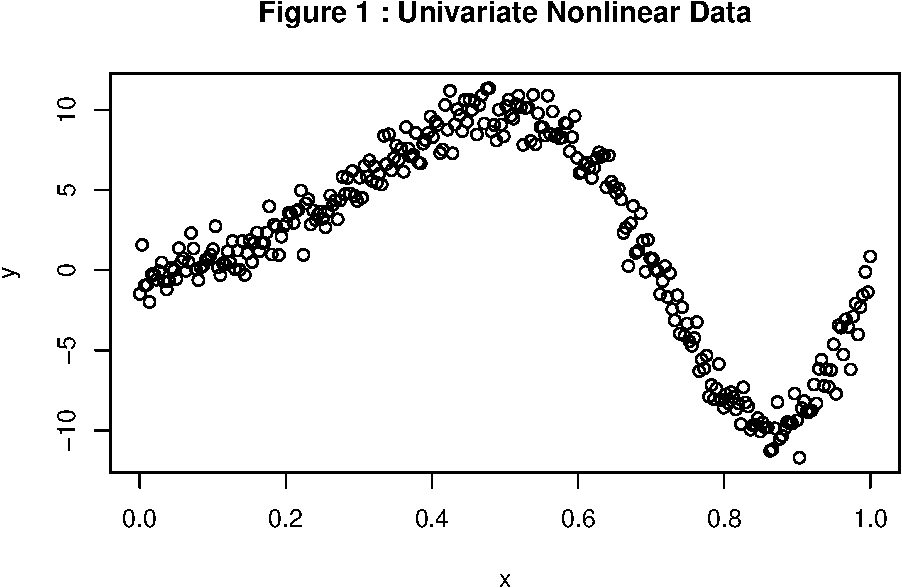
\includegraphics{TBASS_vig_files/figure-latex/unnamed-chunk-4-1.pdf}
\caption{Univariate nonlinear data}
\end{figure}

\begin{figure}
\centering
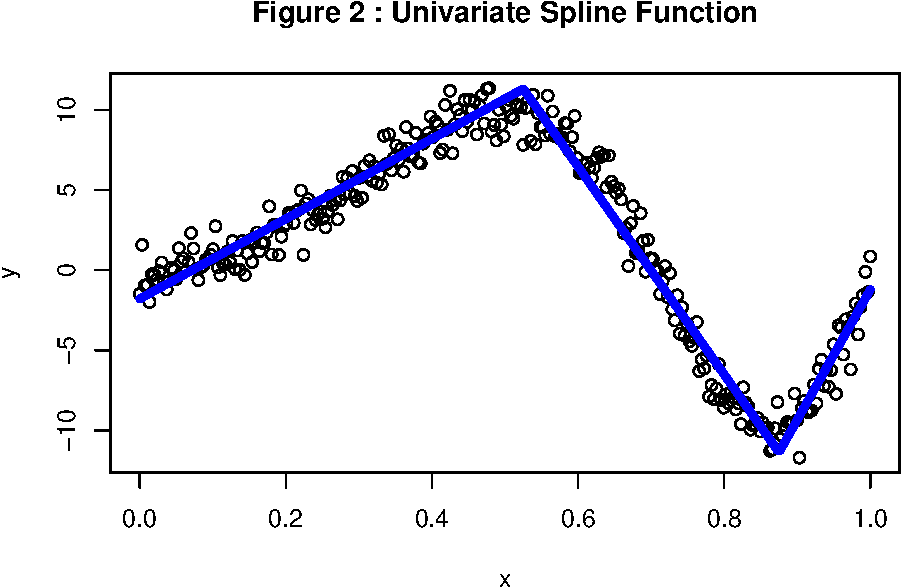
\includegraphics{TBASS_vig_files/figure-latex/unnamed-chunk-5-1.pdf}
\caption{The blue line represents the spline function fit to the data
using three knots}
\end{figure}

\pagebreak

\hypertarget{robust-bmars}{%
\section{Robust BMARS}\label{robust-bmars}}

\hypertarget{overview}{%
\subsection{Overview}\label{overview}}

We want to extend the theory behind frequentist univariate spline
regression to a multivariate Bayesian framework. Moreover, we want to
accurately fit nonlinear data that has outliers. We adopt the Robust
BMARS model based on the standard Gaussian framework used by Denison,
Mallick, and Smith (1998) and Francom et al. (2019) when deriving our
likelihood and full conditional distributions for the parameters.

In the presence of outliers, Gaussian BMARS will attempt to capture the
excess noise by either adding basis functions (overfitting) or inflating
the variance term (\(\sigma^2\)). The Robust BMARS model accounts for
this sensitivity to outliers by avoiding overfitting or variance
inflation when the degrees of freedom (\(\nu\)) are low. When \(\nu\) is
high, the t-distribution closely mimics a normal distribution, so the
Robust BMARS model behaves in a similar way.

The function used to fit the Robust BMARS model in the \texttt{TBASS}
package is the \texttt{tbass()} command (see section
\protect\hyperlink{tbass}{3}).

\hypertarget{likelihood}{%
\subsection{Likelihood}\label{likelihood}}

In creating the Robust BMARS model, we introduce new auxiliary
parameters not used in the Gaussian model (Gelman et al. (2013)).

Similar to Gaussian BMARS, we let \(y_i\) be our dependent variable and
\(\mathbf{x}_i\) be our independent variable. Without loss of
generality, all independent variables \(\mathbf{x}_i\) are scaled from
zero to one (Francom and Sansó (2019)).

In the robust case, the dependent variable \(\bf y\) is modeled as

\begin{equation}
\label{2}
{\bf y} = {\bf B}\boldsymbol{\beta} + {\boldsymbol\epsilon}, \quad {\boldsymbol\epsilon} \sim t_{\nu}\left({\bf 0}, ~ \sigma^2 {\bf I}\right)
\end{equation}

or equivalently,

\begin{equation}
\label{3}
y_i | V_i \sim \mathcal{N}\left({\bf B_{i}}'\boldsymbol{\beta}, ~ \frac{\sigma^2}{V_i}\right).
\end{equation}

We also assume a Gamma prior with shape and rate \(\frac{\nu}{2}\) for
\(V_i\), such that

\begin{equation}
\label{vi}
V_i \sim \Gamma \bigg(\frac{\nu}{2}, ~\frac{\nu}{2}\bigg)
\end{equation}

where \({\bf B}\) represents the matrix of basis functions by column,
\(\boldsymbol \beta\) is the vector of regression coefficients,
\(\boldsymbol\epsilon\) is the error term, \(\nu\) represents the
degrees of freedom in a Student's t-distribution, and
\(\sigma^2\frac{\nu}{\nu - 2}\) is the variance term for \(y_i\).

The basis functions themselves are produced the same way as in the
\texttt{BASS} package by Francom and Sansó (2019).

\hypertarget{priors}{%
\subsection{Priors}\label{priors}}

Our regression coefficients \(\boldsymbol\beta\) follow a Gaussian prior
such that

\begin{equation}
\label{8}
\boldsymbol\beta \sim \mathcal{N} \left( 0,~\tau^2 {\bf I} \right).
\end{equation}

We assume an Inverse-Gamma prior for \(\sigma^2\) with default shape
\(\gamma_1 = 0\) and default rate \(\gamma_2=0\) such that

\begin{equation}
\label{s2}
\sigma^2 \sim IG~(\gamma_1,~\gamma_2).
\end{equation}

For \(\lambda\), we assume a gamma prior such that \(h_1 = h_2= 10\) by
default:

\begin{equation}
\label{lamprior}
\lambda \sim \Gamma \left(h_1, ~h_2\right).
\end{equation}

We use a \(Uniform(0,1)\) prior for \(t_i\) and a discrete uniform prior
for \(s_i\) and \(J_i\).

\hypertarget{posterior}{%
\subsection{Posterior}\label{posterior}}

The full posterior up to a constant is

\begin{equation}
\label{fullpost}
\mathcal{N}\left({\bf B_{i}}'\boldsymbol{\beta}, ~ \frac{\sigma^2}{V_i}\right)~ \Gamma \bigg(\frac{\nu}{2}, ~\frac{\nu}{2}\bigg)~ \mathcal{N} \left( 0,~\tau^2 {\bf I} \right)~ IG~(\gamma_1,~\gamma_2) ~ \Gamma \left(h_1, ~h_2\right)
\end{equation}

\hypertarget{regression-coefficients}{%
\subsubsection{Regression Coefficients}\label{regression-coefficients}}

We can marginalize \(\boldsymbol\beta\) out of the posterior to obtain a
marginal posterior that relies on the regression estimate

\begin{equation}
\label{9}
\boldsymbol{\hat{\beta}} = 
\frac{1}{\sigma^2}
\left( \frac{1}{\sigma^2} {\bf B'VB} + {\tau^{-2}}{{\bf I}} \right)^{-1} {\bf B'} {\bf V}~{{{\bf y}}}
\end{equation}

where \(\tau^2\) is the prior variance for \(\beta_{i}\).

Estimate (\ref{9}) allows us to achieve our t-distributed likelihood
function for the birth step. After marginalizing out
\(\boldsymbol\beta\) and \(\sigma^2\), we can simplify our Likelihood
\(L\) to

\[
L({\bf y}\mid\cdot) \propto \left(\tau^2\right)^{-\frac{M+1}{2}}~ |{\bf V}|^{-1/2}~ \left|{\bf H}^{-1}\right|^{-1/2}\exp\left(-\frac{1}{2}{\bf y'V^{-1}y} \right) \exp\left(-\frac{1}{2}\boldsymbol{\hat{\beta}}'{\bf H^{-1}}\boldsymbol{\hat{\beta}} - 2\boldsymbol{\hat{\beta}}'{\bf B'V^{-1}y}\right)
\]

where \({\bf H} = ({\bf B'V^{-1}B} + \tau^{-2}{\bf I})\).\newline

We then complete the square on the first exponential term using
\({\bf y'~V^{-1}B~ H^{-1}~B'V^{-1}y}\) which simplifies to
\(\boldsymbol{\hat{\beta}}' {\bf H} \boldsymbol{\hat\beta}\) since
\({\bf B'V^{-1}y} = {\bf H}{\boldsymbol{\hat{\beta}}}\) from
(\ref{9}).\newline

From there, we can derive our likelihood:

\[
\begin{aligned}
L({\bf y}\mid\cdot) &= \left(2\pi\tau^2\right)^{-\frac{M+1}{2}}~ |{\bf V}|^{-1/2}~\exp\left(-\frac{1}{2}\left({\bf y'V^{-1}y} - \boldsymbol{\hat{\beta}}' {\bf H} \boldsymbol{\hat\beta}\right)\right)
\exp\left\lbrace-\frac{1}{2}\left(\boldsymbol\beta'{\bf H}\boldsymbol\beta - \boldsymbol\beta'{\bf H}\boldsymbol{\hat{\beta}} - \boldsymbol{\hat{\beta}}'{\bf H}\boldsymbol\beta + \boldsymbol{\hat{\beta}}'{\bf H}\boldsymbol{\hat{\beta}} \right)\right\rbrace\\
&= \left(2\pi\tau^2\right)^{-\frac{M+1}{2}}~ |{\bf V}|^{-1/2}~\exp\left(-\frac{1}{2}\left({\bf y'V^{-1}y} - \boldsymbol{\hat{\beta}}' {\bf H} \boldsymbol{\hat\beta}\right)\right)
\exp\left\lbrace-\frac{1}{2}\left[\left(\boldsymbol\beta -\boldsymbol{\hat{\beta}} \right)'{\bf H}\left(\boldsymbol\beta -\boldsymbol{\hat{\beta}}\right)\right]\right\rbrace\\
&= \left(2\pi\tau^2\right)^{-\frac{M+1}{2}}~ |{\bf V}|^{-1/2}~ \exp\left(-\frac{1}{2}\left({\bf y'V^{-1}y} - \boldsymbol{\hat{\beta}}' {\bf H} \boldsymbol{\hat\beta}\right)\right)~
\mathcal N\left(\boldsymbol\beta \mid \boldsymbol{\hat\beta}, ~{\bf H}^{-1}\right) \left|{\bf H}^{-1}\right|^{-1/2}\left(2\pi\right)^{\frac{M+1}{2}}\\
&= \left(\tau^2\right)^{-\frac{M+1}{2}}  |{\bf V}|^{-1/2}~ \left|{\bf H}^{-1}\right|^{-1/2} \exp\left\lbrace-\frac{1}{2}\left({\bf y'V^{-1}y} - \boldsymbol{\hat{\beta}}' {\bf H} \boldsymbol{\hat\beta}\right)\right\rbrace\\
&= \left(\tau^2\right)^{-\frac{M+1}{2}}  |{\bf V}|^{-1/2}~ \left|{\bf H}^{-1}\right|^{-1/2} \exp\left\lbrace-\frac{1}{2}\left({\bf y'V^{-1}y} - \boldsymbol{\hat{\beta}}' \left({\bf B'V^{-1}B} + \tau^{-2}{\bf I}\right) \boldsymbol{\hat\beta}\right)\right\rbrace
\end{aligned} 
\]

\begin{equation}
\label{like}
\Rightarrow L({\bf y}\mid\cdot) = (\tau^2)^{\frac{M+1}{2}} |{\bf V}|^{-1/2} ~\left|({\bf B'V^{-1}B} +{\tau^{-2}} {\bf I})^{-1}\right|^{-1/2} \exp\bigg\lbrace -\frac{1}{2}\big({\bf y'V^{-1}y} - \boldsymbol{\hat\beta}' ({\bf B'V^{-1}B} +{\tau^{-2}} {\bf I})^{-1}\boldsymbol{\hat\beta}\big) \bigg\rbrace
\end{equation}

Equation (\ref{like}) is the likelihood for the current model with \(M\)
basis functions.\newline

\hypertarget{reversible-jump-markov-chain-monte-carlo-rj-mcmc}{%
\subsection{Reversible-Jump Markov Chain Monte Carlo
(RJ-MCMC)}\label{reversible-jump-markov-chain-monte-carlo-rj-mcmc}}

Like Gaussian BMARS, the robust algorithm adaptively builds, deletes,
and modifies basis functions, sampling candidate knot locations, signs,
interaction degrees, and accepting or rejecting the candidate values
using a RJ-MCMC algorithm.\newline

RJ-MCMC is a generalization of the traditional Metropolis-Hastings
algorithm in the sense that RJ-MCMC allows for parameter dimension
change, allowing for simulation when the number of parameters is
unknown. This is important for BMARS because we want to learn where
knots should be placed and how many basis functions to have in our
model, along with the degree of interaction for our basis functions. We
also want to know if certain basis functions should be added, deleted,
or changed.\newline

Our Robust generalization for the RJ-MCMC algorithm is largely based off
the work by Denison, Mallick, and Smith (1998).\newline

The BMARS model has three possible move types, which is sampled using a
discrete uniform:

\begin{itemize}
\item
  \textbf{Birth}: adding a basis function
\item
  \textbf{Death}: deleting a basis function
\item
  \textbf{Change}: changing a knot, sign, and values of a basis function
\end{itemize}

Once the move type is sampled, the RJ-MCMC algorithm is used to
determine acceptance of that move type.

Our acceptance ratio \(\alpha\) is denoted by

\begin{equation}
\label{TBD}
\alpha = \min\left\lbrace 
1,\
\frac{\pi(\theta') \ S(\theta'\rightarrow\theta)}{\pi(\theta)\ S(\theta\rightarrow\theta')} 
\right\rbrace
\end{equation}

where \(\theta'\) represents the candidate model parameters and
\(\theta\) represents the current model parameters, \(\pi\) is the
likelihood multiplied by the prior, and \(S\) is the proposal to jump
from one model to another.

Section \protect\hyperlink{birth}{2.6} details the RJ-MCMC algorithm for
the birth step in detail. The death and change steps are very similar in
nature.

\hypertarget{birth}{%
\subsection{Birth Step}\label{birth}}

\hypertarget{likelihood-ratio}{%
\subsubsection{Likelihood Ratio}\label{likelihood-ratio}}

Since a basis function is added for the birth step, we have that

\begin{equation}
L({\bf y} \mid {\theta' = M'}) \propto 
\left(\tau^2\right)^{-\frac{M+2}{2}}  |{\bf V}|^{-1/2}~ \left|{\bf H}^{-1}\right|^{-1/2} \exp\left\lbrace-\frac{1}{2}\left(\bf{y'V^{-1}y} - \boldsymbol{\hat{\beta}}' \left(\bf{B'V^{-1}B} + \tau^{-2} {\bf I}\right) \boldsymbol{\hat\beta}\right)\right\rbrace
\end{equation}

Using (\ref{like}), the likelihood ratio
\(\frac{L(\theta')}{L(\theta)}\) is then represented as

\begin{equation}
\label{12}
\frac{L({\bf y} \mid {\theta' = M'=M+1})}{L({\bf y} \mid {\theta = M})} = \frac{\left(\tau^2\right)^{-\frac{M+2}{2}}  |{\bf V}|^{-1/2}~ \left|{\bf H}^{-1}_c\right|^{-1/2} \exp\left\lbrace-\frac{1}{2}\left({\bf y'V^{-1}y} - \boldsymbol{\hat{\beta}}'_{c} \left({\bf B'_{c}V^{-1}B_{c}} + \tau^{-2}{\bf I_{c}}\right) \boldsymbol{\hat\beta}_{c}\right)\right\rbrace}
{\left(\tau^2\right)^{-\frac{M+1}{2}}  |{\bf V}|^{-1/2}~ \left|{\bf H}^{-1}\right|^{-1/2} \exp\left\lbrace-\frac{1}{2}\left({\bf y'V^{-1}y} - \boldsymbol{\hat{\beta}}' \left({\bf B'V^{-1}B} + \tau^{-2}{\bf I}\right) \boldsymbol{\hat\beta}\right)\right\rbrace}\\\\
\end{equation}

where the subscript \(c\) denotes the candidate move type of the
algorithm (a birth step in this case).\newline

The death is very similar to the birth step, with a candidate likelihood
of \(L({\bf y} \mid \theta'=M'=M-1)\). There is no dimension change in
the change step.

\hypertarget{prior-ratio}{%
\subsubsection{Prior Ratio}\label{prior-ratio}}

For the birth step, our prior ratio \(\frac{p(\theta')}{p(\theta)}\) is
of the following form, based on Francom et al. (2019):

\begin{equation}
\label{bprior}
\frac{\lambda}{M+1} ~\bigg(\frac{1}{2}\bigg)^{J} {p\choose J}^{-1} \bigg(\frac{1}{J_{max}}\bigg)~ (M+1)
\end{equation}

where \(\frac{\lambda}{M+1}\) is the prior for the number of basis
functions with \(M\) current knots, \(\big(\frac{1}{2}\big)^{J}\) is the
prior for the signs, \({p\choose J}^{-1}\) is the prior for the number
of possible variable combinations to create basis functions with,
\(\frac{1}{J_{max}}\) is the prior for the number of interactions, and
\(M+1\) is accounting for ordering the basis functions.

\hypertarget{proposal-ratio}{%
\subsubsection{Proposal Ratio}\label{proposal-ratio}}

Our proposal ratio for a birth step
\(\frac{S(\theta'\rightarrow\theta)}{S(\theta\rightarrow\theta')}\) can
be expressed as:

\begin{equation}
\label{bprop}
\frac{\frac{1}{3} \frac{1}{M+1}}{\frac{1}{3} \frac{1}{J_{max}} {p \choose J}^{-1} (\frac{1}{2})^{J}}
\end{equation}

which is effectively the probability of selecting a death step
multiplied by the probability of selecting a specific basis function to
kill, over the probability of proposing the already-proposed basis
function.

The RJ-MCMC algorithm in \texttt{TBASS} calculates the likelihoods,
priors, proposals, and acceptance ratios all on the log scale.

\hypertarget{gibbs-sampling}{%
\subsection{Gibbs Sampling}\label{gibbs-sampling}}

Once the basis function move type is complete, the model parameter
values \(\lambda\), \(V_i\), \(\sigma^2\), and \(\boldsymbol{\beta}\)
can then be sampled using Gibbs Sampling, since the full conditionals
are all closed-form (Denison, Mallick, and Smith (1998)). The Gibbs
Sampling steps shown below are not unique to the birth step as they are
performed after every RJ-MCMC iteration.

Derived from section \protect\hyperlink{priors}{2.3}, the full
conditionals are of the following form:

\begin{equation}
\lambda | \cdot\sim \Gamma\big(h_1 + M, ~h_2 + 1\big)
\end{equation}

\begin{equation}
V_i | \cdot \sim \Gamma\left\lbrace\frac{\nu + 1}{2},~ \frac{1}{2\sigma^2} \sum_{i=1}^{n}{({\bf y} - {\bf X}\boldsymbol\beta)^2}\right\rbrace
\end{equation}

\begin{equation}
\sigma^2 | \cdot\sim IG\left(\gamma_1 + \frac{n}{2}, ~\gamma_2 + \frac{1}{2} \left({\bf y} - {\bf B}\boldsymbol{\beta}\right)' \left({\bf y} - {\bf B}\boldsymbol{\beta}\right)  \right)
\end{equation}

\begin{equation}
\boldsymbol{\beta} | \cdot \sim \mathcal{N}\bigg( \boldsymbol{\hat\beta}, \left({\bf B'V^{-1}B} + \tau^{-2}{\bf I}\right) \bigg)
\end{equation}

where \(\boldsymbol{\hat\beta}\) is denoted in (\ref{9}).\newline

\pagebreak

\hypertarget{tbass}{%
\section{\texorpdfstring{Simulation with
\texttt{tbass()}}{Simulation with tbass()}}\label{tbass}}

We now demonstrate the capabilities of the \texttt{TBASS} package using
the main command, \texttt{tbass()}. The command uses an \texttt{Rcpp}
interface (C++ functions) to optimize computation time. For all
parameter values of this function, please refer to the help
documentation by running \texttt{?tbass} after loading the
package.\newline

\textbf{Software Requirements and Dependencies}

At this time, you must have R Version 4.0.2 (Taking Off Again) or higher
to install and use \texttt{TBASS}.

The package \texttt{mnormt} is REQUIRED in order to use \texttt{TBASS}.
Please run \texttt{install.packages("mnormt")} to install the package.
This dependency will be removed when the package is updated further. No
other dependencies are required.\newline

We begin by loading in the package and setting the seed for
reproducibility. The package can be installed using the following
command: \texttt{devtools::install\_github("aashen12/TBASS")} which
requires installing the package \texttt{devtools}.\newline

When installing \texttt{TBASS}, you may be asked to update packages to a
more recent version. Please update all packages (option 1).

When installing \texttt{RcppArmadillo}, you may be asked to install the
package from sources which need compilation. Please type ``no''.

If you are not asked for these updates, please allow the installation to
proceed normally.\newline

\begin{Shaded}
\begin{Highlighting}[]
\KeywordTok{set.seed}\NormalTok{(}\DecValTok{12}\NormalTok{)}
\KeywordTok{library}\NormalTok{(TBASS)}
\end{Highlighting}
\end{Shaded}

\hypertarget{friedman-function-simulation}{%
\subsection{Friedman Function
Simulation}\label{friedman-function-simulation}}

We fit the Robust BMARS model to the infamous Friedman Function
(Friedman (1991)):

\begin{equation}
\label{fried}
10 ~sin(  \pi x_1 x_2) ~+~ 20(x_3 - 0.5)^2 ~+~ 10x_4 ~+~ 5x_5 
\end{equation}

In R:\newline

\begin{Shaded}
\begin{Highlighting}[]
\NormalTok{f <-}\StringTok{ }\ControlFlowTok{function}\NormalTok{(x) \{}
  \DecValTok{10}\OperatorTok{*}\KeywordTok{sin}\NormalTok{(pi}\OperatorTok{*}\NormalTok{x[,}\DecValTok{1}\NormalTok{]}\OperatorTok{*}\NormalTok{x[,}\DecValTok{2}\NormalTok{]) }\OperatorTok{+}\StringTok{ }\DecValTok{20}\OperatorTok{*}\NormalTok{(x[,}\DecValTok{3}\NormalTok{]}\OperatorTok{-}\NormalTok{.}\DecValTok{5}\NormalTok{)}\OperatorTok{^}\DecValTok{2} \OperatorTok{+}\StringTok{ }\DecValTok{10}\OperatorTok{*}\NormalTok{x[,}\DecValTok{4}\NormalTok{] }\OperatorTok{+}\StringTok{ }\DecValTok{5}\OperatorTok{*}\NormalTok{x[,}\DecValTok{5}\NormalTok{]}
\NormalTok{\} }
\end{Highlighting}
\end{Shaded}

We set our true value of \(\sigma = 1\) and attempt to capture the same
variability in using \texttt{tbass()}.

\begin{Shaded}
\begin{Highlighting}[]
\NormalTok{sigma <-}\StringTok{ }\DecValTok{1} \CommentTok{# TRUE noise sd}
\NormalTok{n <-}\StringTok{ }\DecValTok{1000} \CommentTok{# number of observations}
\NormalTok{x <-}\StringTok{ }\KeywordTok{matrix}\NormalTok{(}\KeywordTok{runif}\NormalTok{(n}\OperatorTok{*}\DecValTok{5}\NormalTok{), }\DataTypeTok{nrow =}\NormalTok{ n, }\DataTypeTok{ncol =} \DecValTok{5}\NormalTok{)}
\NormalTok{y <-}\StringTok{ }\KeywordTok{rnorm}\NormalTok{(n, }\DataTypeTok{mean =} \KeywordTok{f}\NormalTok{(x), }\DataTypeTok{sd =}\NormalTok{ sigma)}
\end{Highlighting}
\end{Shaded}

We then add extra noise to simulate a dataset with outliers, and
categorize them for plotting later.

\begin{Shaded}
\begin{Highlighting}[]
\NormalTok{ind <-}\StringTok{ }\KeywordTok{sample}\NormalTok{(n, }\DataTypeTok{size =} \DecValTok{10}\NormalTok{) }\CommentTok{# convert 10 points to outliers}
\NormalTok{y[ind] <-}\StringTok{ }\KeywordTok{rnorm}\NormalTok{(}\DecValTok{5}\NormalTok{, }\KeywordTok{f}\NormalTok{(x[ind,]), }\DecValTok{15}\NormalTok{)}

\NormalTok{col <-}\StringTok{ }\KeywordTok{rep}\NormalTok{(}\DecValTok{1}\NormalTok{,n) }\CommentTok{# for coloring the outlier points in a later plot}
\NormalTok{col[ind] <-}\StringTok{ }\DecValTok{2}
\end{Highlighting}
\end{Shaded}

From there, we can run the \texttt{tbass()} command with 30000 MCMC
iterations (default 10000). Our first simulation is with \(\nu = 10\)
degrees of freedom to simulate a t-distribution with thicker tails.

\begin{Shaded}
\begin{Highlighting}[]
\NormalTok{nmcmc <-}\StringTok{ }\DecValTok{30000} \CommentTok{#number of iterations}
\NormalTok{tb <-}\StringTok{ }\KeywordTok{tbass}\NormalTok{(x, y, }\DataTypeTok{nu =} \DecValTok{10}\NormalTok{, }\DataTypeTok{nmcmc =}\NormalTok{ nmcmc, }\DataTypeTok{verbose =} \OtherTok{FALSE}\NormalTok{)}
\end{Highlighting}
\end{Shaded}

\hypertarget{results}{%
\subsection{Results}\label{results}}

\hypertarget{overfitting-and-prediction}{%
\subsubsection{Overfitting and
Prediction}\label{overfitting-and-prediction}}

We begin by plotting the number of basis functions throughout the entire
simulation in Figure 3.

\begin{figure}
\centering
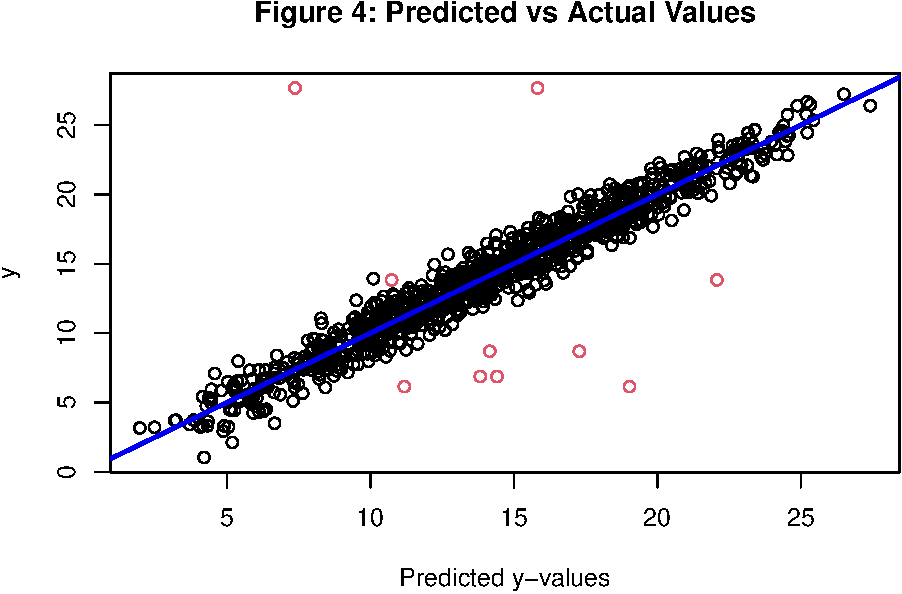
\includegraphics{TBASS_vig_files/figure-latex/unnamed-chunk-11-1.pdf}
\caption{Trace plot of number of basis functions}
\end{figure}

We see that there are 9 basis functions from \texttt{BASS}, indicating
that there was no overfitting in the \texttt{TBASS} model with 10 basis
functions.

We then assess the accuracy of our predicted \(\bf y\) values
(\({\bf X}\boldsymbol\beta\)) vs the actual y-values in Figure 4.

\begin{figure}
\centering
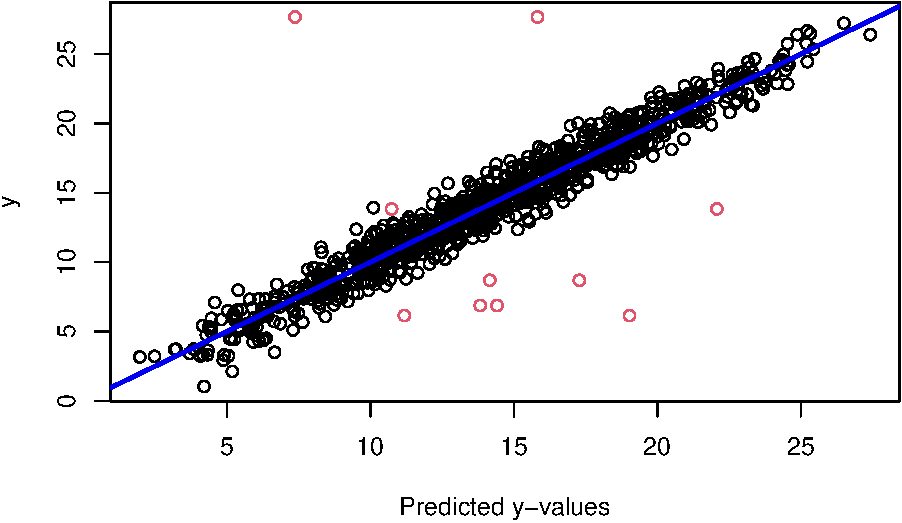
\includegraphics{TBASS_vig_files/figure-latex/unnamed-chunk-12-1.pdf}
\caption{Predicted vs Actual Values}
\end{figure}

We see that the prediction is quite accurate despite the presence of
outliers.

\hypertarget{gibbs-sampling-results}{%
\subsubsection{Gibbs Sampling Results}\label{gibbs-sampling-results}}

We set a burn-in value to the first 50\% of samples.

\begin{Shaded}
\begin{Highlighting}[]
\NormalTok{burn_final <-}\StringTok{ }\NormalTok{nmcmc}\OperatorTok{/}\DecValTok{2}
\NormalTok{burn <-}\StringTok{ }\DecValTok{1}\OperatorTok{:}\NormalTok{burn_final}
\end{Highlighting}
\end{Shaded}

From there, we plot our \(\sigma\) values in Figure 5 to ensure there
was no variance inflation.

\begin{figure}
\centering
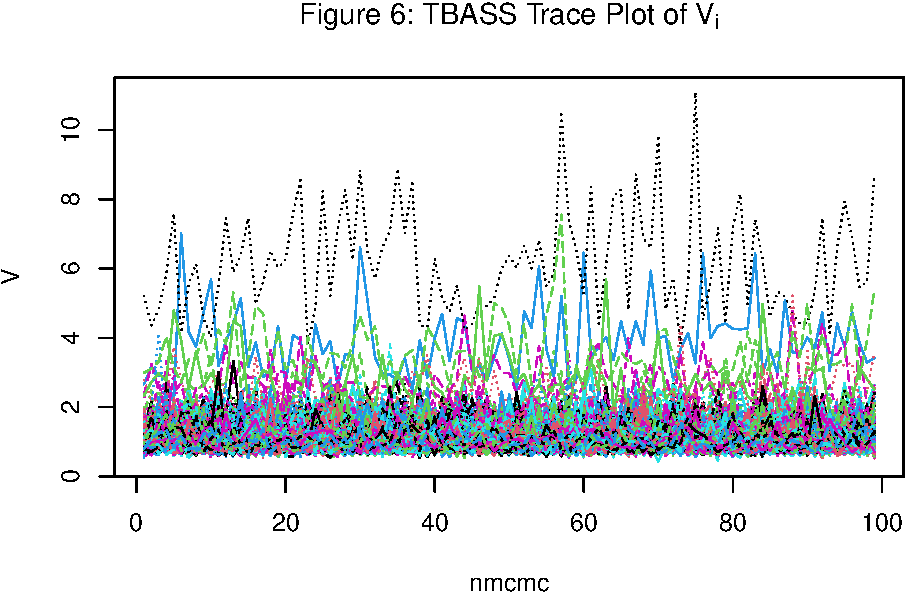
\includegraphics{TBASS_vig_files/figure-latex/unnamed-chunk-14-1.pdf}
\caption{TBASS variance trace plot}
\end{figure}

From this plot, we see that our simulated \(\sigma^2\) values are close
to \(1\), which matches our true value of \(\sigma^2\) when we generated
our data.

We then plot our \(\frac{1}{V_i}\) values to see if the outliers are
accounted for. We thin every \texttt{nmcmc/100} iterations after the
burn-in. See Figure 6.

\begin{figure}
\centering
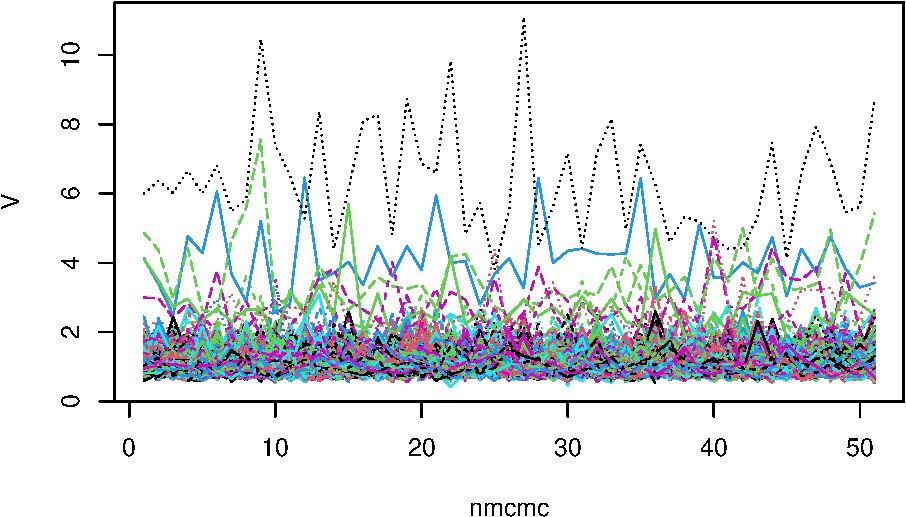
\includegraphics{TBASS_vig_files/figure-latex/unnamed-chunk-15-1.pdf}
\caption{TBASS trace plot of V\_i}
\end{figure}

We see that the peaks in \(V_i\) are accounting for the outliers, while
the majority of \(V_i\) values are in the bottom portion of the plot.

\hypertarget{comparison-with-bass}{%
\subsection{\texorpdfstring{Comparison with
\texttt{BASS}}{Comparison with BASS}}\label{comparison-with-bass}}

To account for the differences in behavior for Robust BMARS
(\texttt{TBASS}) and Gaussian BMARS (\texttt{BASS}), we compare our
results from TBASS to the output from BASS, which assumes a Gaussian
likelihood.

\begin{Shaded}
\begin{Highlighting}[]
\KeywordTok{set.seed}\NormalTok{(}\DecValTok{12}\NormalTok{)}
\KeywordTok{library}\NormalTok{(BASS)}
\NormalTok{b <-}\StringTok{ }\KeywordTok{bass}\NormalTok{(x,y,}\DataTypeTok{nmcmc =} \DecValTok{30000}\NormalTok{) }\CommentTok{# automatically runs 10000 nmcmc iterations}
\CommentTok{# > MCMC Start #-- Sep 23 10:38:08 --# nbasis: 0 }
\CommentTok{# > MCMC iteration 1000 #-- Sep 23 10:38:10 --# nbasis: 11 }
\CommentTok{# > MCMC iteration 2000 #-- Sep 23 10:38:12 --# nbasis: 11 }
\CommentTok{# > MCMC iteration 3000 #-- Sep 23 10:38:13 --# nbasis: 12 }
\CommentTok{# > MCMC iteration 4000 #-- Sep 23 10:38:15 --# nbasis: 11 }
\CommentTok{# > MCMC iteration 5000 #-- Sep 23 10:38:17 --# nbasis: 10 }
\CommentTok{# > MCMC iteration 6000 #-- Sep 23 10:38:19 --# nbasis: 10 }
\CommentTok{# > MCMC iteration 7000 #-- Sep 23 10:38:21 --# nbasis: 10 }
\CommentTok{# > MCMC iteration 8000 #-- Sep 23 10:38:23 --# nbasis: 10 }
\CommentTok{# > MCMC iteration 9000 #-- Sep 23 10:38:24 --# nbasis: 10 }
\CommentTok{# > MCMC iteration 10000 #-- Sep 23 10:38:27 --# nbasis: 10 }
\CommentTok{# > MCMC iteration 11000 #-- Sep 23 10:38:29 --# nbasis: 9 }
\CommentTok{# > MCMC iteration 12000 #-- Sep 23 10:38:31 --# nbasis: 10 }
\CommentTok{# > MCMC iteration 13000 #-- Sep 23 10:38:32 --# nbasis: 10 }
\CommentTok{# > MCMC iteration 14000 #-- Sep 23 10:38:34 --# nbasis: 9 }
\CommentTok{# > MCMC iteration 15000 #-- Sep 23 10:38:36 --# nbasis: 9 }
\CommentTok{# > MCMC iteration 16000 #-- Sep 23 10:38:37 --# nbasis: 9 }
\CommentTok{# > MCMC iteration 17000 #-- Sep 23 10:38:39 --# nbasis: 9 }
\CommentTok{# > MCMC iteration 18000 #-- Sep 23 10:38:41 --# nbasis: 9 }
\CommentTok{# > MCMC iteration 19000 #-- Sep 23 10:38:42 --# nbasis: 9 }
\CommentTok{# > MCMC iteration 20000 #-- Sep 23 10:38:44 --# nbasis: 9 }
\CommentTok{# > MCMC iteration 21000 #-- Sep 23 10:38:46 --# nbasis: 9 }
\CommentTok{# > MCMC iteration 22000 #-- Sep 23 10:38:48 --# nbasis: 9 }
\CommentTok{# > MCMC iteration 23000 #-- Sep 23 10:38:49 --# nbasis: 9 }
\CommentTok{# > MCMC iteration 24000 #-- Sep 23 10:38:51 --# nbasis: 10 }
\CommentTok{# > MCMC iteration 25000 #-- Sep 23 10:38:52 --# nbasis: 11 }
\CommentTok{# > MCMC iteration 26000 #-- Sep 23 10:38:54 --# nbasis: 10 }
\CommentTok{# > MCMC iteration 27000 #-- Sep 23 10:38:56 --# nbasis: 10 }
\CommentTok{# > MCMC iteration 28000 #-- Sep 23 10:38:57 --# nbasis: 10 }
\CommentTok{# > MCMC iteration 29000 #-- Sep 23 10:38:59 --# nbasis: 11 }
\CommentTok{# > MCMC iteration 30000 #-- Sep 23 10:39:01 --# nbasis: 10}
\end{Highlighting}
\end{Shaded}

\hypertarget{bass-basis-functions}{%
\subsubsection{BASS Basis Functions}\label{bass-basis-functions}}

Figure 7 shows that there are also 10 basis functions once the
\texttt{BASS} algorithm is complete, similar to TBASS.

\begin{figure}
\centering
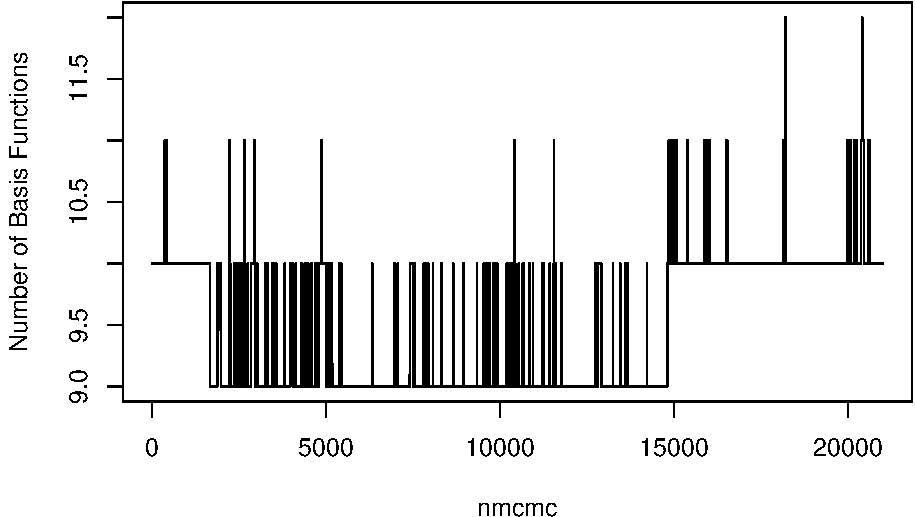
\includegraphics{TBASS_vig_files/figure-latex/unnamed-chunk-17-1.pdf}
\caption{BASS Basis Function Count}
\end{figure}

\hypertarget{bass-variance}{%
\subsubsection{BASS Variance}\label{bass-variance}}

\begin{figure}
\centering
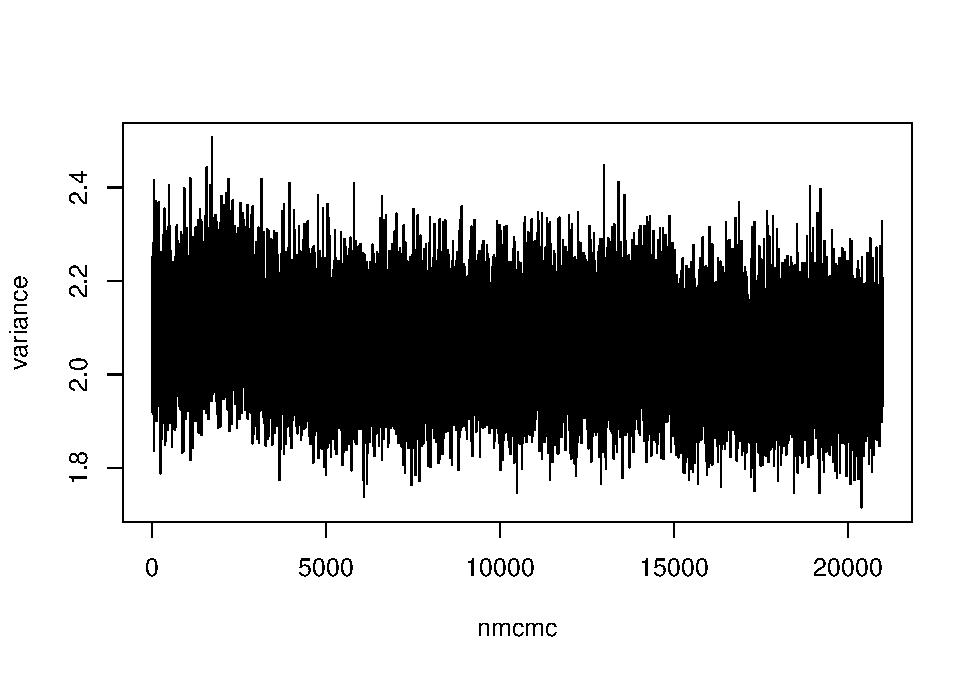
\includegraphics{TBASS_vig_files/figure-latex/unnamed-chunk-18-1.pdf}
\caption{BASS Variance Trace Plot}
\end{figure}

We see that the \(\sigma^2\) from Gaussian BMARS is over two times as
large as the \(\sigma^2\) from \texttt{TBASS}, indicating that Gaussian
BMARS is more sensitive to outliers and will inflate \(\sigma^2\) when
outliers are present.

\hypertarget{conclusion}{%
\section{Conclusion}\label{conclusion}}

We constructed a generalized version of Gaussian Bayesian Multivariate
Adaptive Regression to accommodate data with outliers or data that is
non-Gaussian. This framework provides reliable and accurate parameter
estimation. The R package \texttt{TBASS} adopts this framework from the
original \texttt{BASS} package. These two models have been tested and
compared to show their differences and demonstrate how a low value of
\(\nu\) can emulate the results from a Student's t-distribution.

\hypertarget{references}{%
\section*{References}\label{references}}
\addcontentsline{toc}{section}{References}

\hypertarget{refs}{}
\leavevmode\hypertarget{ref-denison1998bayesian}{}%
Denison, David GT, Bani K Mallick, and Adrian FM Smith. 1998. ``Bayesian
Mars.'' \emph{Statistics and Computing} 8 (4): 337--46.

\leavevmode\hypertarget{ref-francom2019bass}{}%
Francom, Devin, and Bruno Sansó. 2019. ``Bass: An R Package for Fitting
and Performing Sensitivity Analysis of Bayesian Adaptive Spline
Surfaces.'' \emph{Journal of Statistical Software} 2.

\leavevmode\hypertarget{ref-francom2019inferring}{}%
Francom, Devin, Bruno Sansó, Vera Bulaevskaya, Donald Lucas, and Matthew
Simpson. 2019. ``Inferring Atmospheric Release Characteristics in a
Large Computer Experiment Using Bayesian Adaptive Splines.''
\emph{Journal of the American Statistical Association} 114 (528):
1450--65.

\leavevmode\hypertarget{ref-friedman1991multivariate}{}%
Friedman, Jerome H. 1991. ``Multivariate Adaptive Regression Splines.''
\emph{The Annals of Statistics}, 1--67.

\leavevmode\hypertarget{ref-gelman2013bayesian}{}%
Gelman, Andrew, John B Carlin, Hal S Stern, David B Dunson, Aki Vehtari,
and Donald B Rubin. 2013. \emph{Bayesian Data Analysis}. CRC press.

\end{document}
